\section{Communication}

In the Internet of Things, various devices and systems need to exchange information seamlessly.
Industrial environments present unique challenges for communication networks.
eyond environmental challenges, industrial networks must meet strict performance requirements. 
Timeliness is critical, as real-time data transmission ensures efficient and safe automation. 
Deterministic network behavior guarantees predictable response times, while reliability minimizes downtime and operational risks.

Designing a communication network for industrial systems requires careful planning. 
Network size and the number of connected devices determine the scale of infrastructure. 
The mobility of nodes, whether fixed or moving, influences the choice of communication protocols. 
Quality of Service constraints, including latency, throughput, and reliability, must align with operational demands. 
Integration with existing systems poses challenges, as legacy infrastructure must seamlessly connect with modern technologies.
Budget constraints also play a role, influencing technology selection and implementation strategies.

Industrial communication networks handle various types of data traffic.
\begin{definition}[\textit{Cyclic traffic}]
    Cyclic traffic involves periodic transmissions, ensuring continuous process monitoring.
\end{definition}
\begin{definition}[\textit{Acyclic traffic}]
    Acyclic traffic occurs in response to unpredictable events. 
\end{definition}
\begin{definition}[\textit{Multimedia traffic}]
    Multimedia traffic includes images, video streams, and other data-intensive transmissions.
\end{definition}
\begin{definition}[\textit{Backhand traffic}]
    Backhand traffic aggregates data flows from multiple sources, consolidating information for centralized processing and analysis.
\end{definition}

\subsection{Key performance indicators}
\begin{definition}[\textit{Throughput}]
    Throughput refers to the rate at which data can be transmitted over a network link, typically measured in bits per second or bytes per second.
\end{definition}
\noindent The actual throughput depends on the type of link being used, as different technologies offer varying transmission capacities.
\begin{definition}[\textit{Delivery time}]
    Delivery time represents the total time required to transfer a service data unit from the source to the destination.
\end{definition}
\noindent Measured in seconds, it is influenced by multiple factors, including transmission time, propagation time, and the execution time of network protocols.
\begin{definition}[\textit{Minimum cycle time}]
    Minimum Cycle Time defines the shortest duration needed to complete one full cycle within a control loop. 
\end{definition}
\noindent This metric is crucial in real-time systems, where consistent and predictable execution times are essential for maintaining stability and efficiency.
\begin{definition}[\textit{Jitter}]
    Jitter measures the precision and reliability of periodic operations, particularly in time-sensitive applications.
\end{definition}
\noindent Variability in timing can lead to performance issues, making jitter a critical factor in industrial and communication networks that require consistent and predictable timing.

\subsection{Technology}
Defining a communication technology involves several key aspects, starting with the physical infrastructure.

This includes hosts, such as sensors, actuators, PLCs, and SCADA systems, which serve as traffic endpoints. 
Communication links, whether fiber optics, wireless, or wired connections, facilitate data transmission.
Network nodes, including access points, switches, routers, and gateways, manage traffic flow and interconnect various components.

IoT connectivity rarely relies on a single-hop or single-technology approach. 
Instead, it integrates multiple heterogeneous technologies to ensure seamless communication across diverse environments. 
The classification of communication technologies often depends on their range.
\begin{figure}[H]
    \centering
    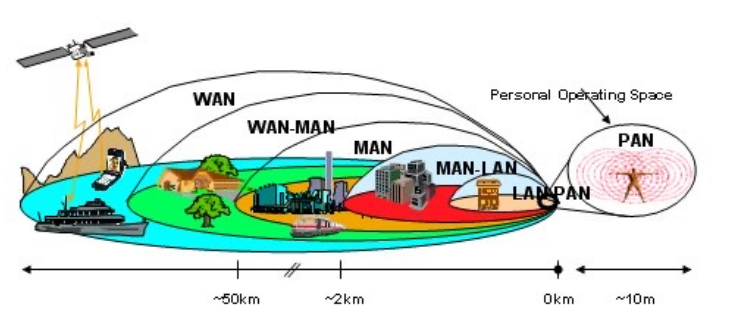
\includegraphics[width=0.5\linewidth]{images/net.png}
    \caption{Connection range}
\end{figure}
Network topology also plays a significant role in communication technology classification. 
Ring topology provides a structured flow of data, while linear chains connect devices sequentially. 
Tree topology enables hierarchical communication, whereas star topology centralizes connections around a single node. 
Mesh networks offer robust, decentralized connectivity, enhancing reliability and redundancy in complex systems.

\subsection{Protocols}
Communication protocols define the set of rules governing the exchange of information between two entities. 
These rules specify aspects such as message format, connection setup and teardown procedures, and the semantics of the transmitted data. 
In IoT communication networks, protocols facilitate packet-based data exchange, similar to how the Internet operates.

Most communication protocols follow a layered architecture, where each layer provides specific services and functionalities to the layers above it. 
This structured approach enhances interoperability, modularity, and scalability in network communication. The primary layers include:
\begin{itemize}
    \item \textit{Application layer}: handles messages exchanged between applications, enabling services such as HTTP, MQTT, and CoAP.
    \item \textit{Transport layer}: manages end-to-end communication through segmentation and reassembly, with protocols like TCP and UDP.
    \item \textit{Network layer}: routes packets across different networks, using IP-based addressing and routing mechanisms.
    \item \textit{Data link layer}: organizes data into frames, ensuring reliable point-to-point or point-to-multipoint transmission.
    \item \textit{Physical layer}: deals with the actual transmission of raw bits over physical media such as wired or wireless connections.
\end{itemize}